\chapter{SAMBA 3}
Este capítulo descreve como são feitas a instalação e a configuração de um servidor samba como controlador de domínio, servidor de impressão e servidor de dados, respeitando as regras de usuários e permissões.

\section{Instalação do samba}

O pacote samba pode ser instalado através do repositório de sistemas da distribuição em que está sendo usado (neste caso Ubuntu 11.04). Primeiro temos que atualizar a base de dados do repositório para que possamos instalar a versão mais atual do samba.

\begin{itemize}
    \item \textbf{\# apt-get update} - Atualiza a base de dados do repositório no Ubuntu.
    \item \textbf{\# apt-get install samba} - Realiza a instalação do pacote samba.
    \item \textbf{\# apt-get install smbclient} - Pacote que mostra as informações do servidor samba e permite acesso de compartilhamentos no windows ou linux a partir de uma máquina linux.
\end{itemize}

\section{SWAT - Gerenciando o samba pelo browser}

Com ele é possível compartilhar impressoras, arquivos, criar usuários, permitir ou restringir acessos, tudo em um ambiente gráfico.

\begin{itemize}
 \item \textbf{\# apt-get install swat} - Instala a ferramenta gráfica swat para o gerenciamento do samba.
    \item \textbf{\$ firefox localhost:901} - Endereço de acesso no browser (neste caso o Firefox) para acessar o swat.
\end{itemize}

Informe o usuário root e sua senha. Como se pode ser na Figura \ref{swat_login}

\begin{figure}[hp]
   	\centering
    \scalebox{1}{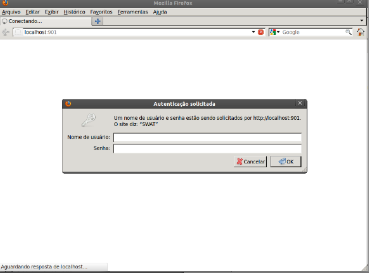
\includegraphics{figuras/swat_login}}
   	\caption{Tela do Login no Swat}
    \label{swat_login}
\end{figure}

Na barra de ferramentas pode se observar as opções de configuração do swat. Da esquerda para direita vemos:

**FIGURA DO SWAT

\begin{itemize}
    \item \textbf{Home} - Documentação do samba
    \item \textbf{Globals} - Variáveis globais de configuração do samba
    \item \textbf{Shares} - Ativar compartilhamentos de diretórios e arquivos
    \item \textbf{Printers} - Compartilhamento de impressoras
    \item \textbf{Wizard} - Escreve as modificações no arquivo smb.conf do samba
    \item \textbf{Status} - Status do servidor com usuário, compartilhamento dos ativos e arquivos abertos
    \item \textbf{View} - Mostra o arquivo smb.conf
    \item \textbf{Password} - Cadastrar o usuário, máquinas e mudar senha dos usuários no servidor
\end{itemize}

\section{Iniciando Samba}

Com todos os componentes instalados o servidor samba pode ser iniciado.

\begin{itemize}
	\item \textbf{\# /etc/init.d/smbd start} - Inicia o samba. Existem outras formas de inicia-lo, como:
		\begin{enumerate}
			\item \textbf{\# service smbd start} - Inicia o samba.
			\item \textbf{\# service smbd stop} - Para o processo do samba.
			\item \textbf{\# service smbd restart} - Finaliza o processo existente e cria outro para o samba.
			\item \textbf{\# /etc/init.d/samba start} - Para iniciar o samba em computadores com Debian 6.
			\item \textbf{\# /etc/init.d/samba restart} - Reiniciar no Debian 6.
		\end{enumerate}
\end{itemize}

\section{Configuração do samba para ser um PDC}

O arquivo de configuração se encontra no diretório /etc, onde está a maioria dos arquivos de configuração dos programas no linux.

\begin{itemize}
	\item \textbf{\# cp /etc/samba/smb.conf $>$ /etc/samba/smb.conf.bkp} - Por motivo de segurança é recomendado fazer um backup do arquivo.
	\item \textbf{\# gedit /etc/samba/smb.conf} - Para editar o arquivo e adicionar as seções, parâmetros e variáveis deve-se abrir o arquivo smb.conf.
	\item \textbf{\# testparm -s /etc/samba/smb.conf.bkp $>$ /etc/samba/smb.conf} - Removerá os comentário para melhor leitura do arquivo. Observação: o arquivo de origem não pode ser o smb.conf pois ele irá se rescrever e o arquivo só conterá a seção [global] vazia.  
\end{itemize}

Agora é necessário inserir, modificar e remover alguns parâmetros na seção [global] para que o samba se comporte como um PDC.
{\raggedright

[global] 

	workgroup = "nome do servidor de domínio" 

	server string = "Título"       

	security = user

	netbios name = "nome que será da netbios do servidor"

	domain master = yes

	domain logons = yes

	enable privileges = yes

	passdb backend = tdbsam
	
	encrypt passwords = true

	preferred master = yes

	local master = yes

	os level = 100

	wins support = yes

	map to guest = Bad User

	panic action = /usr/share/samba/panic-action \%d
}

Explicação das variáveis utilizadas:

\begin{itemize}
	\item \textbf{workgroup} - Nome do servidor de domínio.
	\item \textbf{server string} - Descrição do servidor que aparece na barra de título das janelas do compartilhamento.
	\item \textbf{security} - Tipo de segurança do compartilhamento. Existem os tipos domain, user e share.
		\begin{enumerate}
			\item {share}  - É utilizado quando o compartilhamento será aberto, onde todos os usuários conectados serão guest e sem a necessidade de realizar login.
			\item {user} - Todos os usuários que tentarem se conectar terão que se identificar por meio de um login e uma senha.
			\item {domain} - Quando um servidor de domínio será responsável pela identificação e segurança dos usuários.
		\end{enumerate} 
	\item \textbf{netbios name} - Nome da netbios do servidor.
	\item \textbf{encrypt passwords} - Quando informado a variável "true" as senhas informadas para o servidor serão criptografadas.
	\item \textbf{domain master} - Informa que o servidor samba será o domínio principal da rede.
	\item \textbf{domain logons} - O servidor samba passa a ser um controlador de domínio.
	\item \textbf{enable privileges} - Habilita alguns privilégios no samba. Alguns deles:
		\begin{enumerate}
			\item {SeAddUsersPrivilege} - Adicionar usuários e grupos no domínio 
			\item {SeDiskOperatorPrivilege} - Gerencia os discos compartilhados 
			\item {SeMachineAccountPrivilege} - Adicionar maquinas no domínio 
			\item {SePrintOperatorPrivilege} - Gerencia as impressoras
		\end{enumerate}
	\item \textbf{passdb backend} - Aceita valores smbpasswd ou tdbsam . Define qual será a forma de armazenagem dos registros dos usuários.
		\begin{enumerate}
			\item{smbpasswd} - Segundo (http://www.hardware.com.br/tutoriais/samba-configuracao-avancada/pagina8.html) O smbpasswd é o backend mais simples. Nele, as senhas são salvas no arquivo "/etc/samba/smbpasswd" e são transmitidas de forma encriptada através da rede, com suporte ao sistema NTLM, usado pelas versões contemporâneas do Windows. A vantagem do smbpasswd é que ele é um sistema bastante simples. Embora encriptadas, as senhas são armazenadas em um arquivo de texto, com uma conta por linha.
			\item{tdbsam} - Segundo (http://www.hardware.com.br/tutoriais/samba-configuracao-avancada/pagina8.html) O tdbsam, que usa uma base de dados muito mais robusta, armazenada no arquivo "/var/lib/samba/passdb.tdb" (é justamente este arquivo que o script executado durante a instalação do pacote "samba" no Debian pergunta se deve ser criado).
			\item{Diferença entre smbpasswd e tdbsam} - Segundo (http://www.hardware.com.br/tutoriais/samba-configuracao-avancada/pagina8.html) O tdbsam oferece duas vantagens sobre o smbpasswd: oferece um melhor desempenho em servidores com um grande número de usuários cadastrados e oferece suporte ao armazenamento dos controles SAM estendidos usados pelas versões server do Windows. O uso do tdbsam é fortemente recomendável caso seu servidor tenha mais do que algumas dezenas de usuários cadastrados ou caso você pretenda usar seu servidor Samba como PDC da rede (veja mais detalhes a seguir). Ele é também um pré-requisito caso você precise migrar um domínio NT já existente para o servidor Samba. 
		\end{enumerate}
	\item \textbf{local master} - Define se o servidor será o Master Browser.
	\item \textbf{os level} - Valor que será passado na eleição para definir o mestre da rede. O valor máximo é 100, assim vencendo os valores padrões de "os level" o servidores windows.
	\item \textbf{win support} - Se nmbd será um servidor WINS.
	\item \textbf{map to guest} - Tornar usuário guest todos que não conseguirem se identificar com um login e senha valido.
	\item \textbf{panic action} - Comando que será executado caso o smbd ou nmbd pararem de funcionar.
\end{itemize}

Com todas as variáveis devidamente adicionadas o servidor samba precisa ser reiniciado para que todas as modificações entrem em vigor.

\begin{itemize}
	\item \textbf{\# testparm} - Verifica se existe algum erro de sintaxe no arquivos de configuração no smb.conf
	\item \textbf{\# /etc/init.d/smbd restart} - Reinicia o samba.
	\item \textbf{\# /etc/init.d/nmbd restart} - Reinicia o servidor de nomes do samba.
\end{itemize}

**FIGURA DA SAIDA DO TESTPARM

\section{Cadastro de Usuário}

Os usuários que terão acesso e permissões de login no domínio devem ser criados no servidor linux, onde se encontra o samba. Antes da criação dos usuários normais o usuário root tem que ser cadastrado no samba.

\begin{itemize}
	\item \textbf {\# smbpasswd -a root} - Uma senha terá que ser informada e precisa ser a mesma do usuário no sistema.
\end{itemize}

Cada usuário no sistema deverá conter uma pasta com o nome de "profile.pds". Essa pasta irá conter informações das sessões de logon que o usuário fez no servidor de domínio.

Para automatizar a criação dessa pasta no diretório home dos usuários, cria-se o diretório no /etc/skel.

\begin{itemize}
	\item \textbf{\# mkdir /etc/skel/profile.pds} - O /etc/skel armazena todos os diretórios e arquivos que serão criados juntos com o usuário no sistema.
\end{itemize}

Antes de cadastrá-los no samba eles precisam ser criados no sistema.

\begin{itemize}
	\item \textbf{\# adduser "--disabled-login usuario} - Comando para a criação mais completa de usuário no linux com nome completo, telefone , sem a permissão de login e entre outros dados.
\end{itemize}

Após o usuário ser criado no sistema, ele necessita ser cadastrado no samba.

\begin{itemize}
	\item \textbf{\# smbpasswd -a usuario} - Informe a mesma senha cadastrada no linux.
\end{itemize}

\section{Cadastro de Máquinas}

Da mesma forma que os usuário têm que ser cadastrados no sistema, as máquinas que poderão entrar no domínio também devem ser cadastradas.

As máquinas são cadastradas como usuários normais no linux antes de serem cadastradas no samba, porém sem pasta home e sem bash para login.

\begin{itemize}
	\item \textbf{\# groupadd machine} - Cria o grupo no qual serão adicionadas as máquinas cadastradas para melhor organização dos usuários no linux.
	\item \textbf{\# useradd "--home /dev/null "--shell /bin/false "--group machine computador1\$} - 	Comando para a criação da máquina no sistema linux. Por padrão se adiciona o \$ no final do nome pois é dessa forma que o samba irá identificar que o usuário na verdade é uma maquina. 
	\item \textbf{\# passwd -l computador1\$} - Desativa a mudança da senha para o usuário/máquina.
\end{itemize}

Após a criação do usuário/máquina no sistema agora ele tem que ser cadastrado no samba.

\begin{itemize}	
	\item \textbf{\# smbpasswd -a -m computador1\$} - Cadastra o usuário como uma máquina no samba.
\end{itemize}


\section{Script de Cadastro de Usuários e Máquinas}

Para facilitar a criação e exclusão dos usuários no sistema e no samba, foi feito um script. Com ele é possível criar usuários e máquinas, adicionar usuários em grupos e também excluí-los do sistema.

\textbf{Script smbmanager.sh}

\#!/bin/bash

\#Gabriel Rocha

end=0

help="É NECESSÁRIO TER PERMISSÃO DE ROOT $\backslash$nUSO: smbmanager [OPCAO] [VALOR] $\backslash$n 
$\backslash$nOpções gerais:$\backslash$n -g [VALOR]   Grupo no qual será adicionado a máquina ou usuário  $\backslash$n -m [VALOR]   Nome da máquina a ser cadastrada $\backslash$n -u [VALOR]   Usuário a ser cadastrado no sistema e no samba $\backslash$n -d [VALOR]   Usuário a ser deletado do sistema $\backslash$n -x [VALOR]   Máquina a ser deletada do samba e do sistema"

AddMachine(){

if [ -n "\$machine" ] ; then

    if [ -z "\$group" ] ; then

        useradd "--disabled-login "--home /dev/null "--shell /bin/false \$machine$\backslash$\$ 2$ >$/dev/null \&\& passwd -l \$machine$\backslash$\$ \&\& smbpasswd -a -m \$machine

    fi

    if [ -n "\$group" ]; then
	
        useradd "--disabled-login "--home /dev/null "--shell /bin/false "--group \$group \$machine$\backslash$\$ 

	check=\$(echo \$$?$)

		if [ \$check -eq 0 ]; then
	
 			passwd -l \$machine$\backslash$\$ 2$>$/dev/null \&\& smbpasswd -a -m \$machine 
       fi

    fi        

fi

}

AddUser(){

if [ -n "\$user" ] ; then

    if [ -z "\$group" ] ; then

        adduser \$user 2$>$/dev/null 

        smbpasswd -a \$user

    fi

    if [ -n "\$group" ] ; then

        adduser \$user 2$>$/dev/null

        usermod -g \$user \$group

		check=\$(echo \$$?$)

		if [ \$check -eq 0 ]; then

        	smbpasswd -a \$user

		fi
		
    fi

fi

}

DelMachine(){

if [ -n "\$delmachine" ]; then    

    smbpasswd -x -m \$delmachine

    deluser \$delmachine$\backslash$\$

fi

}

DelUser(){

if [ -n "\$deluser" ]; then    

    smbpasswd -x \$deluser

    deluser \$deluser

fi

}

while getopts "hg:m:u:d:x:" paramentro;

do

   case \$paramentro in

     \ h) echo -e \$help;;

     \ g) group=\$OPTARG ;;

      m) machine=\$OPTARG ;;

      u) user=\$OPTARG ;;

      d) deluser=\$OPTARG ;;

      x) delmachine=\$OPTARG ;;

      *) echo -e \$help; end=1;;

   esac

done

if [[ "\$group" = *'-'* ]] $\|$ [[ "\$machine" = *'-'* ]] $\|$ [[ "\$user" = *'-'* ]] $\|$ [[ "\$deluser" = *'-'* ]] $\|$ [[ "\$delmachine" = *'-'* ]]; then

    echo -e \$help

else

    if [ \$end -ne 1 ] ; then

        AddMachine

        AddUser

        DelMachine

        DelUser

    fi

fi

**FIGURA DO SCRIPT RODANDO

O script tem que ter a permissão de root para que possa ser iniciado.

\begin{itemize}
	\item \textbf{\# chmod +x smbmanger.sh} - Adiciona a permissão de execução ao script.
	\item \textbf{\# cp smbmanager.sh /usr/sbin/} - Transferindo o script para a pasta /usr/sbin/ o script poderá ser iniciado em qualquer caminho que o usuário esteja.
\end{itemize}

\section{Migração dos Usuários Administradores e Users do Linux para o Windows}

Para que o Windows possa reconhecer um grupo de usuários administradores do linux como Power Users e Domain Users deve se mapear os grupos pelo RID dos mesmos.

Primeiro é necessário saber qual o ID dos principais grupos do Windows.

*****TABELA RID WIKI SAMBA*******

RID (Relative Identifier) 

Domain Admins RID=512 

Domain Users RID=513 

Domain Guests RID=514

\begin{enumerate}
	\item \textbf{\# net groupmap list} - Liste os grupos existentes mapeados, caso não tenha o grupo siga o passo 2.		
	\item \textbf{\# net groupmap add ntgroup="Domain Admins" rid=512 unixgroup=admin} - Irá mapear o grupo admin para o grupo Domain Admins do windows.
	\item \textbf{\# net groupmap add ntgroup="Domain Users" rid=513 unixgroup=users} - Mapea o grupo users com o Domain Users do windows.
\end{enumerate}

\begin{itemize}
	\item \textbf{\# net groupmap delete ntgroup="Domain Admins"} - Caso queira remover um mapeamento de grupo.
	\item \textbf{\# net groupmap modify ntgroup="Domain Admins" rid=512 unixgroup=admin} - Caso tenha necessidade de modificar um mapeamento.
\end{itemize}

Dessa forma, se o usuário logar com os usuários que estejam no grupo admin em algum terminal windows no domínio, ele terá permissões de administrador.

\section{Perfis Moveis}

Para que as configurações e personalizações do perfil do usuário no windows sejam salvas é necessário a criação de um perfil móvel no servidor samba. 
A vantagem de se utilizar um perfil móvel é que não existe a obrigatoriedade de se realizar backup na máquina do usuário, pois os arquivos são salvos no servidor, sendo assim é só o usuário fazer o login em outra máquina windows que o seu perfil e os seus dados serão migrados para o novo computador. Porém o perfil móvel tem um problema que é a quantidade de dados armazenados. Se o número de usuários e dados de cada um for muito grande, cria-se a necessidade de ter um servidor com muito espaço e uma rede muito bem estruturada. 

Para ativar a configuração de perfil móvel no samba deve-se adicionar no [global] 

\textbf	{logon path = $\backslash$$\backslash$\%L$\backslash$Profiles$\backslash$\%U}

\textbf {logon home = $\backslash$$\backslash$\%L$\backslash$Profiles$\backslash$\%U}

\textbf	{logon drive = H:}

\begin{itemize}
	\item \textbf{logon path} - Serve para indicar o caminho onde vão ficar os perfis no Windows XP/Vista/7 
	\item \textbf{logon home} - Indica o caminho para os perfis em versões mais antigas do Windows, como 95/98.
	\item \textbf{logon drive} - Unidade que será mapeada com o caminho $\backslash$$\backslash$servidor$\backslash$profiles$\backslash$"nome do usuário" no Windows.
\end{itemize}

Como a estrutura da rede do IFF Bom Jesus é composta por Windows XP/7 e Ubuntu 11.04 ou superior temos a opção de não adicionar a variável "logon home" 

Agora precisamos deletar todas as pastas do diretório home e trocar a sua permissão 

\begin{itemize}
	\item \textbf{\# mkdir /var/samba/usuario}
	\item \textbf{\# chmod 1777 -R /var/samba/usuario}
\end{itemize}

Todo usuário que fizer login no servidor irá criar automaticamente uma pasta com o seu nome e com toda a estrutura do perfil como Desktop, Meus documentos. Com a permissão 1777 o samba se encarrega de permitir somente acesso ao usuário logado, onde o 1 é uma permissão especial. 

Os diretórios criados podem ficar em compartilhamento para o usuário que será mapeado na unidade H no windows.

[profiles] 

	path = /var/samba/usuario 
	
	writeable = yes 
	
	browseable = no 
	
	create mask = 0600 
	
	directory mask = 0700 
	
	available = yes 

\begin{itemize}
	\item \textbf {path} - Caminho da pasta que vai ser compartilhada.
	\item \textbf {writeable} - Permite a escrita no diretório e nos arquivos.
	\item \textbf {browseable} - Define se o compartilhamento poderá ser visto na pasta principal do compartilhamento ou somente pelo endereço completo.
	\item \textbf {create mask} - Força a criação dos arquivos com a permissão 0600, assim somente os donos do arquivo poderão alterar os arquivos.
	\item \textbf {directory mask} - Criação dos diretórios com permissão 0700.
	\item \textbf{available} - (Yes/No) Se o compartilhamento estará acessível ou não no servidor.
\end{itemize}

**FIGURA DO PERFIL MOVEL NO LINUX

\section{Compartilhamento de Arquivos}

O compartilhamento de arquivos é dado pela adição de seções no arquivo smb.conf.

[Diretoria]

path = /media/diretoria

read only = no

valid users = +diretoria

force group = diretoria

create mask = 0770

directory mask = 0770

browseable = no

\begin{itemize}
	\item \textbf{[Diretoria]} - Nome do compartilhamento que será mostrado no servidor.
	\item \textbf{path} - Caminho onde se encontra o diretório no servidor.
		\begin{enumerate}
			\item {\$ mkdir} - Cria uma pasta no servidor. Exemplo: mkdir pasta .
			\item {\# chmod} - Define as permissões do arquivo. Exemplo: \# chmod 774 /pasta\_criada - Essas permissão definem que o usuário proprietário do diretório e todos os usuário do seu grupo terão acesso total ao mesmo e seus arquivos e que os outro usuário poderão apenas listar os arquivos que se encontram no diretório.
			\item {\# chown} - Define qual será o usuário e grupo proprietário do diretório ou arquivo. Exemplo: \# chown usuario.grupo /diretorio .
		\end{enumerate} 
	\item \textbf{read only} - Define se o compartilhamento estará com permissão de somente leitura ou não.
	\item \textbf{Valid users} - Define quais usuários e grupos poderão acessar o compartilhamento. O símbolo de + define que o nome inserido esta se referindo a um grupo de usuários.
	\item \textbf{force group} - Força qual será o grupo proprietário dos arquivos criados no compartilhamento.
	\item \textbf{create mask} - Permissão dos arquivos que forem criados ou inseridos no compartilhamento
	\item \textbf{directory mask} - Permissão dos diretórios do compartilhamento
	\item \textbf{browseable} - Define se o compartilhamento poderá ser visualizado na janela do compartilhamento do servidor.
\end{itemize}

Existem outras variáveis que podem ser adicionadas em um compartilhamento de arquivos dependendo da necessidade.

\begin{itemize}
	\item \textbf{invalid users} - Lista de usuários e grupos que não terão acesso.
	\item \textbf{guest ok} - Permite que qualquer usuário acesse a pasta.
	\item \textbf{veto files} - Impede que certos arquivos sejam transferidos para o servidor.
	\item \textbf{write list} - Lista dos usuários que poderão gravar e fazer alterações nos arquivos e diretórios compartilhados.
	\item \textbf{read list} - Lista dos usuários que só poderão ler e listar os arquivos e diretórios compartilhados.
	\item \textbf{host deny} - Ip`s ou faixa de ips que não podem conectar ao servidor.
	\item \textbf{hosts allow} - Ip`s ou faixas de ips que podem conectar ao compartilhamento.
\end{itemize}

\textbf{Exemplo da aplicação de algumas delas}

[Backup]

write list = usuario1 \# Somente o usuario1 terá permissão de escrita no compartilhamento.

read list = usuario2 \# O usuario2 só poderá ler e listas os arquivos e diretórios desse compartilhamento.

host allow = 192.168.1.2-192.168.1.20 \# Somente os ip's que estiverem entre 192.168.1.2 e 192.168.1.20 poderão acessar esse compartilhamento.

veto files = *.tmp, *.doc \# Não será permitido inserir esses tipos de arquivos no compartilhamento. 

**FIGURA DO COMPARTILHAMENTO NO SERVIDOR

\section{Script Logon}

Para que os mapeamentos de unidades e alguns códigos sejam executados de forma automática nos usuários logados o samba fornece a opção na seção [global]. 

\begin{itemize}
	\item {logon script = \%G.bat } - Com essa variável adicionada, o sistema irá buscar o script com o nome do grupo primário do usuário. Trabalhar com o grupo é mais fácil de se gerenciar pois o mesmo script serve para mais de um usuário. O uso do \%U é um complicador, já que cada seria necessário criar um script para cada usuário do sistema.
\end{itemize}

Exemplo: 

\textbf{Usuário logado : usuário}

\textbf{Grupo primário : grupo}

\textbf{Script a ser procurado : grupo.bat}

Esse script precisa estar compartilhado no smb.conf para que possa ser executado. 

	[netlogon] 

		path = /var/samba/scripts 

		read only = yes 

		browseable = no 
		

%\begin{itemize}
%	\item \textbf{read only} - O compartilhamento só terá a permissão de somente leitura.
    %\item \textbf{browseable} - Define se o compartilhamento será visível ou não
%\end{itemize}

O local onde foi definido que irá conter os scripts e os arquivos (/var/samba/scripts), tem que ter a permissão 1775. 

\begin{itemize}
	\item \textbf{\# mkdir -p /var/samba/scripts} - Cria a pasta onde estarão os scripts.
	\item \textbf{\# chmod 1775 /var/samba/scripts} - Permissão de execução dos scripts.
\end{itemize}

Exemplo de um dos scripts 

diretoria.bat 

\textbf{net use x: $\backslash$$\backslash$servidor$\backslash$diretoria}

**FIGURA DO MAPEAMENTO AUTOMÁTICO 

\section{Compartilhamento de Impressoras}

O compartilhamento de impressora é a publicação das impressoras instaladas no servidor para que outras máquinas que estão na rede possam acessar e imprimir sem precisar da conexão local na impressora.

Para compartilhar as impressoras com o samba deve-se adicionar na seção [global] 

[global]

printing = cups

load printers = yes

\begin{itemize}
	\item \textbf{printing} - Define qual o programa será utilizado para gerenciar as impressões 
	\item \textbf{load printers} - Carrega as impressoras
\end{itemize}

O samba utiliza o cups que é o gerenciador de impressoras mais comum para o linux.

\begin{itemize}
	\item \textbf{\#smbd -b $|$ grep CUPS} - Para saber se o pacote samba instalado é compatível com o CUPS. A saída deve ser algo como "HAVE CUPS"
\end{itemize}

Caso o cups não esteja instalado.

\begin{itemize}
	\item \textbf{\#apt-get install cups} - Instala todos os pacotes necessários para o funcionamento do cups.
	\item \textbf{\$ firefox localhost:631} - Interface gráfica para gerenciar as impressoras.
	\item \textbf{\# /etc/init.d/cupsys restart} - Reinicia o serviço do cups
\end{itemize}

***FIGURA DO CUPS PELO BROWSER***

Habilitando o compartilhamento de impressora

[printers]

print ok = yes

guest ok = yes

path = /var/spool/samba

browseable = yes

\begin{itemize}
	\item \textbf{path} - Esse caminho é onde ficarão os spools de impressão. Esse diretório é criado automaticamente pelo samba e deve ter a permissão 777.
	\begin{enumerate}
		\item \textbf{chmod 777 -R /var/spool/samba}
	\end{enumerate}
\end{itemize}

Dessa forma ao acessar o servidor irão aparecer todas as impressoras instaladas.

\section{Instalação automática dos drive da impressora}

Para conectar-se a uma impressora compartilhada é necessário a instalação dos drivers da mesma. 

Um problema é como esses drivers são armazenados e instalados, já que uma das formas de instalar esses drivers é ir até o computador com o instalador em cd ou pen-drive e realizar a instalação manualmente, porém em uma grande rede se perde muito tempo com a locomoção e instalação. A solução desse problema é a instalação automática dos drivers, e com a utilização do samba os drivers serão instalados assim que o usuário tentar conectar a impressora.

Adiciona no [global]

\begin{itemize}
	\item \textbf{enable privileges = yes} - Permite privilégios a usuários
\end{itemize}

Criar um compartilhamento não visível onde ficará os drivers das impressoras.

[print\$]

path = /var/lib/samba/printers

read only = yes

write list = root

inherit permissions = yes

\begin{itemize}
	\item \textbf{path} - Local onde os drivers serão instalados
	\item \textbf{write list} - Usuários ou grupos que terão permissão de escrita
	\item \textbf{inherit permissions} - Se os arquivos irão herdar as permissões da pasta.
\end{itemize}

Se o caminho apontado pelo path não existir ele terá que ser criado com as permissões necessárias.

\begin{itemize}
	\item \textbf{\# mkdir -p /var/lib/samba/printers}
	
	\item \textbf{\# cd /var/lib/samba/printers}
	\item \textbf{\# mkdir WIN40 W32X86} - Essas pastas são os locais onde ficarão os drivers das impressoras, o WIN40 para sistemas Windows 95/98/ME e o W32X86 Windows NT/2000/XP.
	\item \textbf{\# chmod 2775 WIN40 W32X86} - Permissões especiais para instalar os drivers nos usuários.
	\item \textbf{\# net -S localhost -U root -W BATTOUSAI-SHARE rpc rights grant 'BATTOUSAI-SHARE$\backslash$root' SePrintOperatorPrivilege} - Irá definir que o usuário root terá todas os privilégios necessários para gerenciar as impressoras.
\end{itemize}

Com as permissões, usuários e impressoras configuradas, os drivers têm que ser passados para o servidor.

\begin{enumerate}
	\item \textbf{Acessar a maquina com um usuário local} - 	\ref{login_windows_local}
	\begin{figure}[ht]
	   	\centering
	    \scalebox{1}{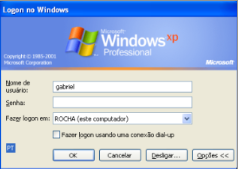
\includegraphics{figuras/login_windows_local}}
	   	\caption{Tela do Login no Windows localmente}
	    \label{login_windows_local}
	\end{figure}	
	
	\item \textbf{Informar o endereço do servidor} - \ref{server_ip}
	\begin{figure}[ht]
	   	\centering
	    \scalebox{1}{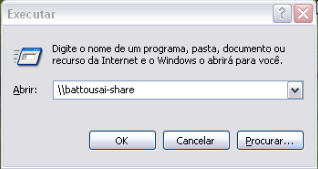
\includegraphics{figuras/server_ip}}
	   	\caption{IP do servidor de compartilhamento}
	    \label{server_ip}
	\end{figure}
	
	\item \textbf{Informar o usuario root e sua senha} - \ref{root_password}
	\begin{figure}[ht]
	   	\centering
	    \scalebox{1}{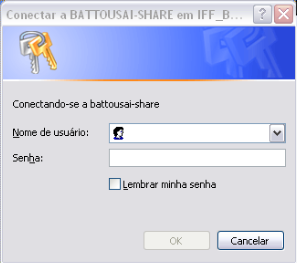
\includegraphics{figuras/root_password}}
	   	\caption{IP ou Netbios do servidor de compartilhamento}
	    \label{root_password}
	\end{figure}
	
	\item \textbf{Acessar a pasta 'Impressoras e aparelhos de fax'} -\ref{impressora_aparelho_fax}
	\begin{figure}[ht]
	   	\centering
	    \scalebox{1}{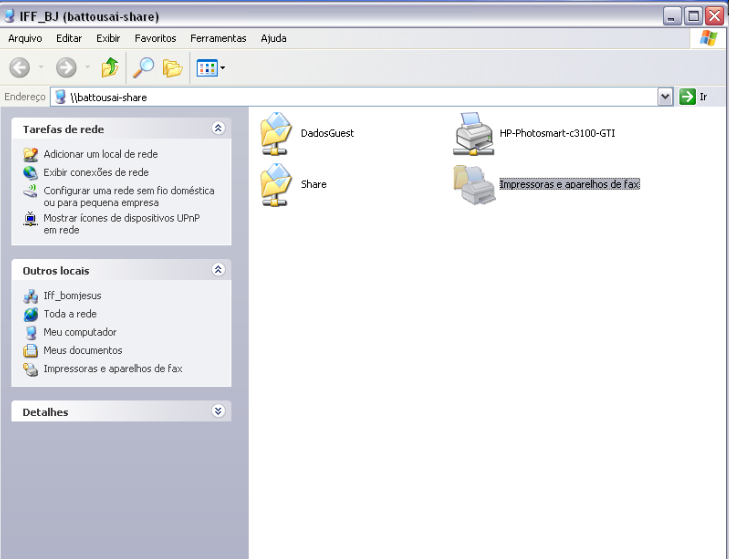
\includegraphics{figuras/impressora_aparelho_fax}}
	   	\caption{Impressoras e aparelhos de fax compartilhados}
	    \label{impressora_aparelho_fax}
	\end{figure}
	
	\item \textbf{Clique na opção Arquivos -$>$ Propriedade do servidor} - \ref{propriedade_servidor}
	\begin{figure}[ht]
	   	\centering
	    \scalebox{1}{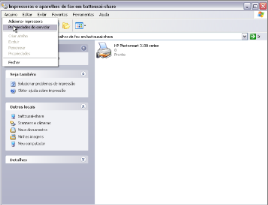
\includegraphics{figuras/propriedade_servidor}}
	   	\caption{Propriedades do servidor de impressão}
	    \label{propriedade_servidor}
	\end{figure}
	
	\item \textbf{Aba Driver -$>$ Adicionar} - \ref{adicionar_driver}
	\begin{figure}[ht]
	   	\centering
	    \scalebox{1}{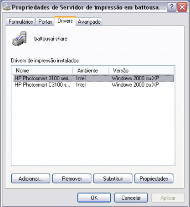
\includegraphics{figuras/adicionar_driver}}
	   	\caption{Adicionar driver ao servidor de impressão}
	    \label{adicionar_driver}
	\end{figure}
	
	\item \textbf{Selecionar o driver da impressora que deve ser copiado para o servidor} - \ref{selecionar_driver}
	\begin{figure}[ht]
	   	\centering
	    \scalebox{1}{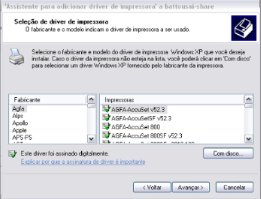
\includegraphics{figuras/selecionar_driver}}
	   	\caption{Selecionar o driver que será copiado para o servidor de impressão}
	    \label{selecionar_driver}
	\end{figure}
	
	\item \textbf{Selecionar os SO dos drivers} - \ref{selecionar_so}
	\begin{figure}[ht]
	   	\centering
	    \scalebox{1}{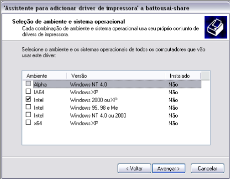
\includegraphics{figuras/selecionar_so}}
	   	\caption{Selecionar os Sistemas Operacional que o driver será compatível}
	    \label{selecionar_so}
	\end{figure}
	
	\item \textbf{Botão direito na impressora Propriedades} - \ref{propriedade_impressora}
	\begin{figure}[ht]
	   	\centering
	    \scalebox{1}{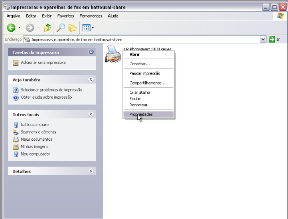
\includegraphics{figuras/propriedade_impressora}}
	   	\caption{Propriedade da impressora do compartilhamento}
	    \label{propriedade_impressora}
	\end{figure}
	
	\item \textbf{Selecione a opção 'Não', se selecionar o SIM o driver será instalado somente na maquina local} - \ref{opcao_nao}
	\begin{figure}[ht]
	   	\centering
	    \scalebox{1}{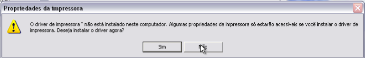
\includegraphics{figuras/opcao_nao}}
	   	\caption{Opção para não instalar o driver naquele momento}
	    \label{opcao_nao}
	\end{figure}
	
	\item \textbf{Aba Avançado} - \ref{aba_avancado}
	\begin{figure}[ht]
	   	\centering
	    \scalebox{1}{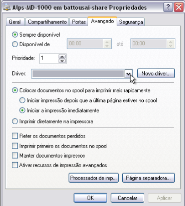
\includegraphics{figuras/aba_avancado}}
	   	\caption{Aba onde será feito o link da impressora com o driver}
	    \label{aba_avancado}
	\end{figure}
	
	\item \textbf{Selecione o drive que será vinculado a impressora} - \ref{aba_avancado}
	
	\item \textbf{Logar com o usuário do domínio no qual será mapeada a impressora} - \ref{login_dominio}
	\begin{figure}[ht]
	   	\centering
	    \scalebox{1}{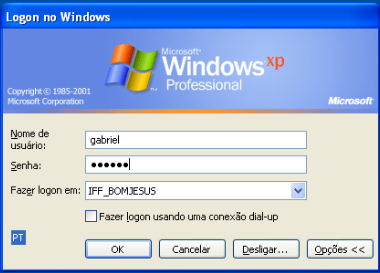
\includegraphics{figuras/login_dominio}}
	   	\caption{Logar no domínio}
	    \label{login_dominio}
	\end{figure}
	
	\item \textbf{Selecione a impressora no servidor} - \ref{selecionar_impressora_servidor}
	\begin{figure}[ht]
	   	\centering
	    \scalebox{1}{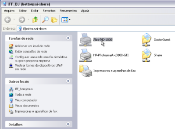
\includegraphics{figuras/selecionar_impressora_servidor}}
	   	\caption{Selecionar a impressora que será mapeado no usuário logado}
	    \label{selecionar_impressora_servidor}
	\end{figure}
	
	\item \textbf{Impressora instalada no usuário} - \ref{impressora_compartilhada}
	\begin{figure}[ht]
	   	\centering
	    \scalebox{1}{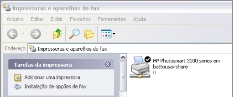
\includegraphics{figuras/impressora_compartilhada}}
	   	\caption{Impressora instalada no usuário}
	    \label{impressora_compartilhada}
	\end{figure}
	
\end{enumerate}

\section{Ingressando o Windows XP no Domínio}

\section{Ingressando o Linux no Domínio}
